\section{Introducción}
En la actualidad, la WWW presenta una cantidad ingente de
información. Un problema al que nos enfrentamos es que esta
información es difícil de procesar y extraer automáticamente, ya que
la inmensa mayoría de esta información está destinada a ser leída por
humanos. Mientras existen esfuerzos, como la web semántica, para
codificar toda esa información de una manera más formal y tratable por
computadoras; hoy por hoy, no es posible acceder a la mayor parte de
la información de la web por medio de procedimientos automáticos.

En este contexto surge aAUTOMATOR\cite{aAUTOMATOR}, una herramienta
creada por el grupo SING para la extracción de información de la
web. Se usa especialmente en el ámbito bioinformático para extraer
información estructurada a partir de información no estructurada
presente en la web. Un uso típico consiste en extraer información de
un portal, combinarlo con información de otra web y mostrar los
resultados con un HTML personalizado.

aAUTOMATOR ofrece un entorno de ejecución para unos
agentes software llamados robots. Los robots visitan varias páginas y
extraen la información deseada, todo ello siguiendo su
especificación. Un robot se especifica por un XML que se puede
producir manualmente o con una herramienta visual.

El uso de XML es adecuado para comunicar la herramienta visual con
aAUTOMATOR, pero dista mucho de ser ideal para su uso directo. Está
más orientado a facilitar su interpretación por aAUTOMATOR que a ser
creado directamente por programadores. Hay ocasiones en las que se
prefiere prescindir de la herramienta visual. Por ejemplo, un
programador desearía poder invocar directamente aAUTOMATOR en sus
programas, pero se ve enfrentado a la complejidad de tener que crear
la especificación XML de un robot.

aAUTOMATOR se trata de una herramienta Java. Aun siendo una plataforma
con muchos usuarios, sería adecuado poder ofrecer esta funcionalidad a
otras plataformas. Consideramos, por lo tanto, muy útil permitir que
aAUTOMATOR sea usado por clientes de otras plataformas.

\subsection{Objetivos}

El presente PFC, \emph{DARE}, está dirigido a suplir estas
carencias. Para ello se han de cumplir los siguientes objetivos:

\begin{itemize}
  \item Facilitar la creación robots. Para ello se diseñará e
    implementará un nuevo lenguaje de programación de propósito
    específico. Este lenguaje permitirá la especificación de los
    robots de manera más concisa y sin perder poder expresivo. Es
    decir, no se perderá funcionalidad con respecto al XML. El
    lenguaje deberá estar destinado a programadores, aunque no se
    descarta su uso por usuarios de alto nivel.

  \item Ofrecer aAUTOMATOR como servicio. Se debe permitir el acceso
    de la funcionalidad de aAUTOMATOR desde el mayor número de
    plataformas. El servicio debe estar orientado a ser consumido por
    software, no directamente por usuarios finales. A mayores el
    servicio debe ser fácilmente escalable, desde ejecución local
    hasta ejecución en un cluster o en la nube.

  \item Crear librerías para consumir el servicio. Se crearán varías
    librerías para facilitar el consumo de aAUTOMATOR como
    servicio. De este modo, se verificará que el servicio ofrecido es
    integrable en varias plataformas.
\end{itemize}

\subsection{Soluciones adoptadas}

A continuación se exponen las tecnologías y técnicas que se han
considerado oportunas para realizar los objetivos propuestos.

\subsubsection{Lenguaje específico de dominio}
Lenguaje específico de dominio, o
DSL\cite{DSL}\footnote{Domain Specific Language}, es un lenguaje
de programación dirigido a un dominio de problema
particular. Gracias al empleo de una DSL consideramos que se ha
abordado con éxito el objetivo de facilitar la creación de robots
por parte de programadores.

Para la implementación de la DSL se ha empleado Ruby\cite{RUBY},
más concretamente su variante JRuby. Hemos implementado, pues, una
DSL interna\cite{DSL}.

\subsubsection{Servicio REST}

Servicio REST. Se ha expuesto aAUTOMATOR vía HTTP siguiendo el estilo
arquitectónico REST\cite{REST}\footnote{\emph{Representational state
    transfer}}.

El uso de HTTP nos permite ofrecer aAUTOMATOR al mayor número de
plataformas. HTTP es un protocolo bien soportado y esto facilita el
acceso del servicio en el mayor número de plataformas.

REST es la filosofía subyacente en el protocolo HTTP. REST define una
serie de restricciones: el estado y la funcionalidad de un servicio
son abstraídos en recursos, son accesibles a través de una sintaxis
uniforme para definir direcciones, un conjunto limitado de verbos para
acceder a y modificar representaciones de los recursos; más un
protocolo cliente-servidor, sin estado y cacheable.  Estas
restricciones proporcionan una serie de beneficios en cuanto a
expansibilidad y escalabilidad, así como facilitan la implementación
de clientes.

Tanto las características de HTTP como REST nos han permitido ofrecer
con garantías aAUTOMATOR como servicio, facilitando en gran medida la
escabilidad del servicio.

Para realizar la implementación del servicio se han empleado varias
tecnologías y lenguajes de programación basados en la
JVM\footnote{\emph{Java Virtual Machine}}:
\begin{description}
\item[JAX\_RS\cite{JAXRS}\footnote{\emph{Java API for RESTful Web
      Services}}:] Se trata de un \emph{API} que facilita la creación
  de servicios web siguiendo el estilo arquitectónico REST.
\item[Clojure\cite{JOY}:] Se trata de un lenguaje dinámico
  implementado sobre la JVM. Es ante todo un lenguaje de programación
  funcional\cite{FUNCTIONAL} con un énfasis especial en la
  programación concurrente. Es un dialecto de Lisp\cite{LISP},
  ofreciendo mecanismos avanzados como macros. Se ha empleado en la
  implementación interna del servidor, ofreciéndonos una alta
  productividad.
\item[MongoDB\cite{MONGO}:] Es una base de datos NoSQL\cite{NOSQL} de
  alto rendimiento y escalable. Nos ha ofrecido un modelo de datos
  conveniente para el problema junto a facilidades para una mayor
  escalabilidad futura.
\end{description}

%\subsubsection{Despliegue en la nube}
%%TODO make it happen
%La implementación del sistema se ha realizado de modo que es posible
%su escalado dinámico en numerosos proveedores de infraestructura en la
%nube. Se ha realizado un despliegue a modo de prueba en
%AWS\footnote{\emph{Amazon Web Services}}. Hemos podido comprobar de
%este modo la escabilidad del servicio.
%
%Se ha considerado importante ofrecer herramientas que ofrezcan la
%automatización del despliegue y el redimensionamiento del servicio,
%siguiendo una filosofía DevOps\cite{DEVOPS}. Clave para poder seguir
%esta filosofía y permitir en el futuro el despliegue de DARE en nuevos
%proveedores se ha empleado:
%
%\begin{itemize}
%  \item jclouds\cite{JCLOUDS}. Se trata de una librería para Java que nos abstrae
%    sobre los detalles de los entornos en nube más típicos. En el
%    momento de escribir este documento, soporta más de 30 proveedores.
%  \item Pallet\cite{PALLET}. Se trata de una plataforma para la
%    automatización de infraestructura tanto para la nube, servidores o
%    máquinas virtuales.
%\end{itemize}

\subsubsection{Librerías cliente}

Se han creado librerías para el consumo del servicio REST implementado
tanto para Java como Python.

Para implementar la librería cliente en Java hemos utilizado la misma
librería que en el lado de servidor, JAX-RS. Esto ha facilitado la
implementación en gran medida, pero no despejaba las incógnitas en
cuanto a interoperabilidad entre plataformas.

Al implementar una librería de acceso en Python queríamos demostrar
que era posible crear librerías en otras plataformas sin problemas de
interoperabilidad. Podemos afirmar que el enfoque REST empleado ha
sido satisfactorio en ese sentido, pudiendo crear una librería
equivalente funcionalmente a la librería en Java.

Además se ha implementado una interfaz de línea de comandos para
facilitar el acceso al servicio. Se ha implementado haciendo uso de la
librería cliente en Python, dado que hemos considerado excesivo el
tiempo de arranque de la JVM.

\subsection{Descripción del sistema}

DARE está compuesto de los siguientes módulos:

\begin{itemize}

  \item DARE-util: Es un cajón de sastre donde se encuentran diversas
    funciones de utilidad usadas por varios otros módulos.

  \item minilanguage: Este módulo es el encargado de implementar el
    lenguaje específico de dominio. Aparte de por el servicio
    implementado se puede usar directamente por otros programas
    Java. Está implementado en JRuby y Java.

  \item DARE-domain: Contiene las clases que forman el dominio de
    datos del sistema. Facilita una comprensión conceptual del
    sistema, ya que únicamente contiene lógica de negocio. A la hora
    de obtener datos del sistema de almacenamiento, instancias de
    clases de este módulo son creadas. Está implementado en Java.

  \item DARE-workers: Es clave para lograr la escabilidad del
    sistema. Está compuesto por una parte cliente que lanza peticiones
    de ejecución a aAUTOMATOR. La parte servidor, de ahora en adelante
    \emph{worker}, interpreta esas peticiones y hace el trabajo
    correspondiente. Uno o varios de estos workers pueden estar
    lanzados en función de las necesidades de escalabilidad y
    fiabilidad necesarias.

    Los workers pueden estar en el nodo local o repartidos por todo el
    cluster. La parte cliente es capaz de descubrirlos y repartir la
    carga de peticiones entre los workers. Aparte comprueba
    continuamente el estado de salud de los workers para que el
    servicio continúe funcionando aun en la presencia de errores en
    los workers.

    Tanto la parte servidor como cliente están implementadas en
    Clojure.

  \item DARE-backend: Es el encargado de comunicarse con la base de
    datos MongoDB tanto para leer como para escribir los objetos
    definidos en DARE-domain. Recibe también peticiones de ejecución
    para aAUTOMATOR. Para llevarlas a acabo utiliza la parte cliente
    de DARE-workers.

    Está implementado en Clojure.

  \item DARE-war: Este módulo es el encargado de implementar el
    servicio. Se trata de una aplicación web Java, por tanto puede
    desplegarse en cualquier servidor de aplicaciones JEE y/o
    contenedor de servlets.

    Siguiendo el patrón MVC\footnote{Modelo Vista Controlador}, este
    modelo es el responsable de la parte de vista y controlador. El
    modelo sería DARE-domain junto a DARE-backend ofreciendo servicios
    de persistencia y ejecución.

    Está diseñado para poder ejecutar numerosas instancias
    simultáneamente, ya que se sigue una filosofía
    \emph{share-nothing}. Para ello nos hacemos valer de las
    características sin estado de REST. Es decir, podemos tener varios
    servidores web ejecutándose en distintos nodos. Está implementado
    en Java.

  \item DARE-web: Este módulo se utiliza para facilitar el despliegue
    de la aplicación. Incluye el contenedor de servlets
    Jetty\cite{JETTY} embebido. Jetty es un contenedor de servlets
    ligero, por lo que es especialmente adecuado para lanzar numerosas
    instancias de la aplicación. Está implementado en Clojure.

  \item DARE-python: Este módulo implementa la librería cliente para
    Python, así como la aplicación de línea de comandos. La aplicación
    de línea de comandos emplea la librería para llevar a cabo su
    funcionalidad. Como es lógico está implementado en Python.

\end{itemize}

\subsection{Visión sistema}

Veamos a continuación un diagrama que muestra un ejemplo de despliegue
de DARE ---ver figura \ref{deployment_example},
pág.~\pageref{deployment_example}---. Podemos apreciar equipos
clientes que se comunican utilizando el protocolo HTTP con DARE. Estos
equipos pueden utilizar alguna de las librerías clientes presentadas
en este proyecto o haber creado su propia librería o aplicación.

Dentro de lo que sería DARE hay tres tipos de nodos:

\begin{itemize}
  \item Un nodo con un balanceador de carga. Para DARE recomendamos
    utilizar nginx\cite{NGINX} como proxy inverso. Este nodo repartirá
    las peticiones entre todos los nodos que estén ejecutando
    DARE-web.
  \item Nodos con el componente DARE-web. Estos nodos atienden
    peticiones HTTP. Si la petición implica una ejecución, se manda
    una solicitud de ejecución a uno de los nodos que tenga
    DARE-worker instalado. Preferiblemente se elegirá el que tenga
    menor carga en ese momento.
  \item Nodos con el componente DARE-worker. Estos nodos reciben las
    peticiones de ejecución vía TCP.
  \item Sistema de almacenamiento. En el caso que se nos ocupa hemos
    empleado MongoDB\cite{MONGO}. Es el punto responsable de almacenar
    el estado del sistema. Todos los procesos ejecutando DARE-web
    carecen de estado: es decir, cada petición se puede dirigir a
    cualquiera de los procesos DARE-web.
\end{itemize}

El ejemplo de despliegue presentado en el diagrama no deja de ser más
que un ejemplo. Se podrían colocar, por ejemplo, los procesos
DARE-worker en los mismos nodos que los procesos DARE-web. En la
sección de instalación ---\ref{local_installation},
pág.~\pageref{local_installation}--- se instalan todos estos elementos
en el mismo nodo. Esa es una buena opción para comenzar, luego según
las necesidades van aumentando se pueden ir añadiendo más nodos con
los tipos de procesos que son más requeridos.

\begin{landscape}
  \begin{figure}[hbp]
    \begin{center}
      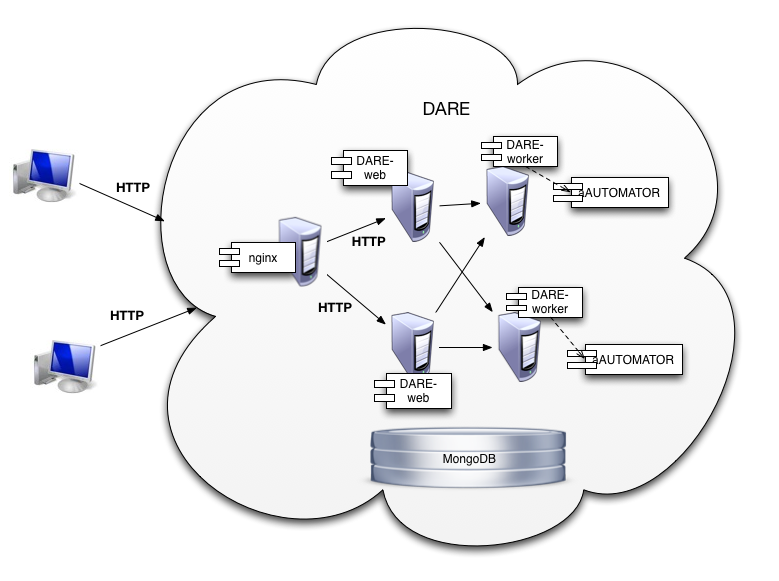
\includegraphics[width=1.4\textwidth]{example-deployment.png}
    \end{center}
  \caption{Ejemplo Despliegue}\label{deployment_example}
  \end{figure}
\end{landscape}

\subsection{Organización de la documentación}

A lo largo de la documentación se emplearán distintos diagramas
siguiendo la notación UML\cite{UML}. La documentación del proyecto se
presenta en único volumen que contiene tres capítulos:

\begin{description}

    \item[Memoria.] Consta de una introducción al presente
      proyecto. Debería servir para alcanzar una visión general del
      mismo.
    \item[Manual Técnico.] Contiene el análisis, diseño y pruebas del
      presente proyecto. Debería transmitir una visión más detallada
      del mismo, así de las decisiones tomadas.

      En el análisis se expondrá la problemática a la que nos
      enfrentamos. Nos apoyaremos en el uso de diagramas de caso de
      uso para indicar la funcionalidad requerida.

      En el diseño expondremos una visión más detallada del sistema,
      procurando entender su funcionamiento. Nos apoyaremos en el uso
      de diagramas de componentes y de clases para transmitir el
      diseño del proyecto. También se comentarán las tecnologías
      empleadas, las alternativas que se sopesaron y el modo en el que
      se implantaron.

      En las pruebas se mostrará un listado de las diversas pruebas
      presentes en el proyecto. Hay presentes tanto pruebas unitarias
      como de integración. Los tests aquí presentados son
      automatizados para evitar posibles regresiones futuras.

    \item[Manual Usuario.] Contiene el manual de administrador y
      usuario del presente proyecto.

      El manual de administrador explica cómo desplegar el proyecto
      tanto en un equipo local como en un cluster.

      El manual de usuario explica como utilizar el servicio ofrecido
      orientado a una audiencia técnica. Se explicará como usar la
      aplicación de línea de comandos.
\end{description}

Junto a la documentación se incluirá un CD con el siguiente contenido:

\begin{verbatim}
.
├── all.policy
├── build-common.xml
├── build.xml
├── DARE-backend
├── DARE-domain
├── DARE-java
├── DARE-python
├── DARE-util
├── DARE-war
├── DARE-web
├── DARE-workers
├── docs
├── ivyconf-local.xml
├── ivyconf-public.xml
├── ivysettings-default-chain.xml
├── ivysettings-m2-publication.xml
├── ivysettings.xml
├── lib
├── minilanguage
├── Procfile
└── target

12 directories, 9 files
\end{verbatim}

Aparte se puede obtener la última versión del proyecto mediante git:

\verb+git clone https://github.com/ogf/DARE+.

De este modo se puede acceder a las actualizaciones realizadas después
de que se haya entregado el proyecto.

\section{Planificación y presupuesto}
\subsection{Planificación temporal}
En su totalidad el proyecto se ha realizado en 640 horas, mientras que
la previsión del proyecto fueron 440 horas. La planificación temporal
inicial se encuentra en el anteproyecto ---ver el anexo
\ref{ANTEPROYECTO}, pág.~\pageref{ANTEPROYECTO}---. El desvío se ha
producido sobre todo a que se escogieron tecnologías todavía no
conocidas y que hubo que aprender. Además se evaluaron más tecnologías
de las previstas a la hora de realizar el proyecto.

A continuación mostramos una tabla con el tiempo empleado en las
tareas planificadas, seguida del diagrama de Gantt de las mismas.

\begin{landscape}
  \begin{figure}[hbp]
    \begin{center}
      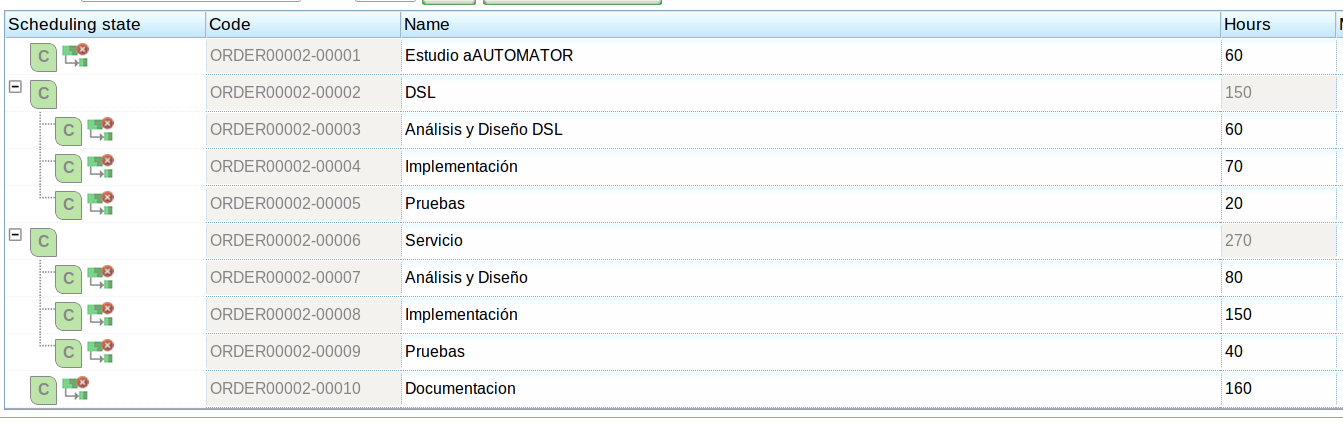
\includegraphics[width=1.4\textwidth]{tasks-structure.png}
    \end{center}
  \caption{Desglose Tareas}\label{tasks_structure}
  \end{figure}
\end{landscape}
\begin{landscape}
  \begin{figure}[hbp]
    \begin{center}
      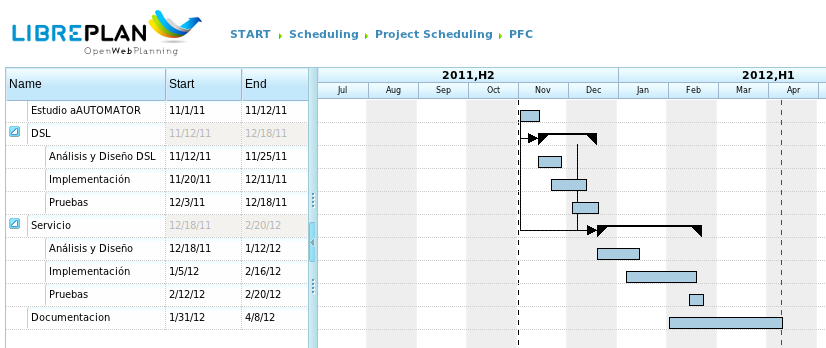
\includegraphics[width=1.4\textwidth]{gantt-diagram.png}
    \end{center}
  \caption{Diagrama Gantt}\label{gantt_diagram}
  \end{figure}
\end{landscape}
\subsection{Presupuesto}

A continuación mostramos los costes fijos ---tabla \ref{fixed_costs},
pág.~\pageref{fixed_costs}--- y los costes humanos estimados ---tabla
\ref{human_costs}, pág.~\pageref{human_costs}---. En cuanto a los
costes humanos sólo hemos indicado las horas empleadas. Hemos
preferido no imputar un precio a cada hora porque es completamente
circunstancial y en el caso de un proyecto fin de carrera irreal.
\newpage
\begin{table}[hbp]
\begin{tabularx}{\textwidth}{X r}
\textbf{Recurso} & \textbf{Precio} \\\hline
Ubuntu 11.10 & 0€ \\
OpenJDK Server VM 1.6\_023 & 0€ \\
Eclipse Indigo & 0€ \\
\XeLaTeX{}  & 0€ \\
Emacs 23 & 0€ \\
MongoDB 2.0.3 & 0€ \\
Sony Vaio VPCZ11X9E (amortizado) & 450€ \\ \hline
\textbf{Total} & 450€ \\
\end{tabularx}
\caption{Costes Fijos}
\label{fixed_costs}
\end{table}

\begin{table}[hbp]
\begin{tabularx}{\textwidth}{X r}

\textbf{Recurso} & \textbf{Horas} \\ \hline
Analista/Diseñador & 200 horas\\
Programador & 220 horas \\
Documentación & 160 horas \\
Pruebas & 60 horas \\ \hline
\textbf{Total} & 640 horas \\
\end{tabularx}
\caption{Costes Humanos}
\label{human_costs}
\end{table}

\section{Conclusiones y posibles ampliaciones}

\subsection{Conclusiones}

La realización de una herramienta para ser utilizada por otros
programadores es una sensación novedosa. Normalmente nuestros
desarrollos están orientados a un usuario final, lo que requiere un
especial énfasis en el diseño de la interacción con el usuario.
Desarrollar hacia un público más técnico nos presenta otra serie de
desafíos: ofrecer abstracciones adecuadas, ni muy concretas, ni
demasiado genéricas; facilitar la comprensión del producto creado,
poca utilidad tiene una librería si no es comprendida; facilitar su
uso, de poco sirve una librería si tiene asociada un sinfín de
dependencias y salvedades.

El empleo de una DSL\footnote{\emph{Domain Specific Language}} ha
demostrado ser una técnica útil y provechosa. La creación de una DSL
permite expresar la solución a un problema recurrente, de una manera
clara, concisa y con la mínima redundancia. Creo, por tanto, que es
una herramienta, que en el contexto adecuado, puede proporcionar altas
cotas de abstracción y una mejora de productividad considerable. En el
caso concreto de este proyecto se ha empleado una DSL interna. Lo
cual, nos ha permitido ofrecer una solución satisfactoria en un tiempo
reducido. Ruby ha demostrado una gran maleabilidad, demostrando ser
una buena opción para la implementación de la DSL internas. Como
inconveniente, cabe citar que la elección de una DSL interna ha
dificultado, en mayor medida, la personalización de los errores del
lenguaje creado. Aun así, dado el ámbito reducido del mismo, considero
que no presenta mayor problema para los usuarios técnicos a los que va
dirigido el proyecto.

A mayores, he podido familiarizarme con el funcionamiento de varias
bases de datos de lo que se ha venido en llamar movimiento
\emph{NoSQL}. He podido observar que bajo esta etiqueta se esconde una
panoplia de base de datos con características radicalmente
diferentes. Más que nada se podrían definir por lo que no son: la
típica base de datos relacional --- MySQL, PostgreSQL, Oracle, etc---.
Sin desdeñar la utilidad de las bases de datos relacionales y sus
grandes aportaciones, a veces otro tipo de base de datos son más
adecuadas para un problema. Creo que, en este sentido, la experiencia
de este proyecto ha sido fundamental para ampliar mis recursos a la
hora de enfrentarme a nuevos problemas.

Aunque ya conocía el estilo arquitectónico REST, ahora he alcanzado un
conocimiento más elevado de la filosofía del mismo. Desde aquí, no
puedo más que recomendar la lectura de la disertación doctoral de
Roy~Fielding\cite{REST}. Es un documento que ofrece una visión
perspicaz, mediante la sucesiva introducción de restricciones
arquitectónicas, de los principios que han guiado el desarrollo de
HTTP.

Este proyecto también ha ayudado a adentrarse en el mundo de la
programación funcional\cite{FUNCTIONAL}. Este paradigma se presenta
especialmente útil ante los retos de un presente y futuro en el que
las mejoras de rendimiento pasan por aprovechar el mayor número de
CPUs disponibles. Clojure, en concreto, ha ofrecido una experiencia
agradable y ha roto muchas asunciones provenientes de mis experiencias
con lenguajes OO\footnote{\emph{Object Oriented}}. Además me voy con
la sensación de que la programación funcional, con la reducción de
efectos laterales que conlleva, es una de las mejores herramientas que
disponemos en la batalla por limitar la complejidad a la hora de
construir y comprender sistemas.
%
%Otro campo en el que el proyecto ha ayudado ha sido adentrarme en el
%mundo de la \emph{Cloud Computing}. Hemos comprobado que el uso de
%AWS\footnote{\emph{Amazon Web Services}}, nos ha ofrecido flexibilidad
%a la hora de escalar el servicio. Así podemos ofrecer el servicio,
%tanto a un público reducido, como a un público amplio, simplemente
%añadiendo nuevas instancias dinámicamente. Pallets, nos ha ofrecido
%una gran facilidad para automatizar el despliegue y el
%redimensionamiento del servicio. Mientras que jclouds nos ofrece
%flexibilidad futura, permitiéndonos portabilidad a otros proveedores
%en el futuro.

Como no todo puede ser positivo, cabe destacar que la integración de
tantas tecnologías ha presentado sus retos y una mayor complejidad que
la deseada a la hora de hacer el \emph{build} del sistema. También
señalar que la programación distribuida presenta su propio conjunto de
dificultades y retos, presentado una mayor dificultad que las partes
más secuenciales del proyecto. Destacaría que, aparte de la típica
faceta de desarrollo que ha contemplado el proyecto, la administración
de sistemas ha supuesto un componente altamente enriquecedor.

Por último señalar que el presente proyecto ha contemplado la
evaluación y aprendizaje de numerosas tecnologías y técnicas. Siempre
resulta satisfactorio aprender nuevas tecnologías, al tiempo que se
muestran fundamentales para ofrecer una solución adecuada. Considero
que en la informática es altamente importante un proceso de
aprendizaje continuo. En este sentido, el proyecto ha sido un éxito,
equipándome con nuevas técnicas y tecnologías que a buen seguro serán
de utilidad en un futuro.

\subsection{Posibles ampliaciones}

Hay una serie de ampliaciones que se podrían llevar a cabo:

\begin{itemize}
  \item Herramienta para instalar automáticamente DARE en varios
    nodos, preferiblemente en AWS\footnote{\emph{Amazon Web Services}}.
  \item Crear una herramienta que facilite la creación de robots
    basados en la DSL creada. Debería ofrecer auto-completado,
    coloreado de sintaxis, marcado de errores, etc.
  \item Añadir nuevas librerías para otros lenguajes: JavaScript, Ruby
    y C.
  \item Sería relativamente sencillo que el servicio ofreciese soporte
    a otras librerías de \emph{web scraping} como Beautiful
    Soup\cite{SOUP}, WWW::Mechanize\cite{MECHANIZE} o
    Hpricot\cite{HPRICOT}.
  \item Robots privados. Actualmente por defecto todos los robots y
    los resultados son públicos. Esto facilita compartir información y
    la facilidad de uso. Aun así, podría ser útil para algunos casos
    la creación de usuarios y restringir el acceso a la información
    generada.
  \item \label{MASHUP_REF} Crear una \emph{mashup}\cite{MASHUP} web. Sería
    interesante crear una aplicación web basada en JavaScript que
    facilitase la creación y ejecución de robots por parte de usuarios
    finales. Esta aplicación haría peticiones hacia el servicio.
  \item Paquetizar DARE. Sería interesante crear paquetes para las
    distribuciones Linux más populares como Debian, Ubuntu, Red Hat,
    etc. Así facilitaríamos el despliegue de nuevas instalaciones de
    DARE.
\end{itemize}
